\documentclass[a0paper,fleqn]{betterposter/betterposter}
\usepackage{hyperref}
\usepackage{hyperxmp}
\usepackage{pythonhighlight}
\usepackage[
    type={CC},
    modifier={by},
    version={3.0},
]{doclicense}
\lstset{
language = Python,
backgroundcolor={\color[gray]{.95}},
breaklines = true,
basicstyle=\fontsize{30}{32}\selectfont\ttfamily,
commentstyle = {\itshape \color[cmyk]{1,0.4,1,0}},
keywordstyle = {\bfseries \color[cmyk]{0,1,0,0}},
stringstyle = {\ttfamily \color[rgb]{1,0,0}},
}

\begin{document}
\betterposter{

	\maincolumn{

		3D plotting and mesh analysis through a streamlined interface for the Visualization Toolkit (VTK)
	}{

		\qrcode{images/qrcode}{images/smartphoneWhite}{
			\textbf{Take a picture} to
			\\download the full paper
		}
		% Smartphone icon
		% Author: Freepik
		% Retrieved from: https://www.flaticon.com/free-icon/smartphone_65680

	}

}{

	
\includegraphics[width=\textwidth]{images/logo}\\
	VTK implements an object-oriented approach to 3D visualization,
	and PyVista adheres to that underlying structure to provide an API that
	expands on VTK's data types. These expanded, wrapped types hold methods and
	attributes for quickly accessing scalar arrays, inspecting properties of
	the dataset, or using filtering algorithms to transform datasets.
	PyVista wrapped objects have a suite of common filters ready for immediate
	use directly on the objects. These filters are commonly used algorithms in the
	VTK library that have been made more accessible by binding a method to control
	that algorithm directly onto all PyVista datasets, providing a shared set of
	functionality. Through the use of these bound filtering methods, powerful VTK
	algorithms can be leveraged and controlled via keyword arguments designed to
	be intuitive for novice users.

	At its core, PyVista is a pure Python helper module for VTK
	that interfaces back to VTK data objects through NumPy
	and direct array access adhering to VTK's object-oriented approach to
	3D visualization.
	The PyVista Python package provides an accessible and intuitive interface back
	to the VTK library to facilitate rapid prototyping, analysis, and visual
	integration of spatially referenced datasets.

	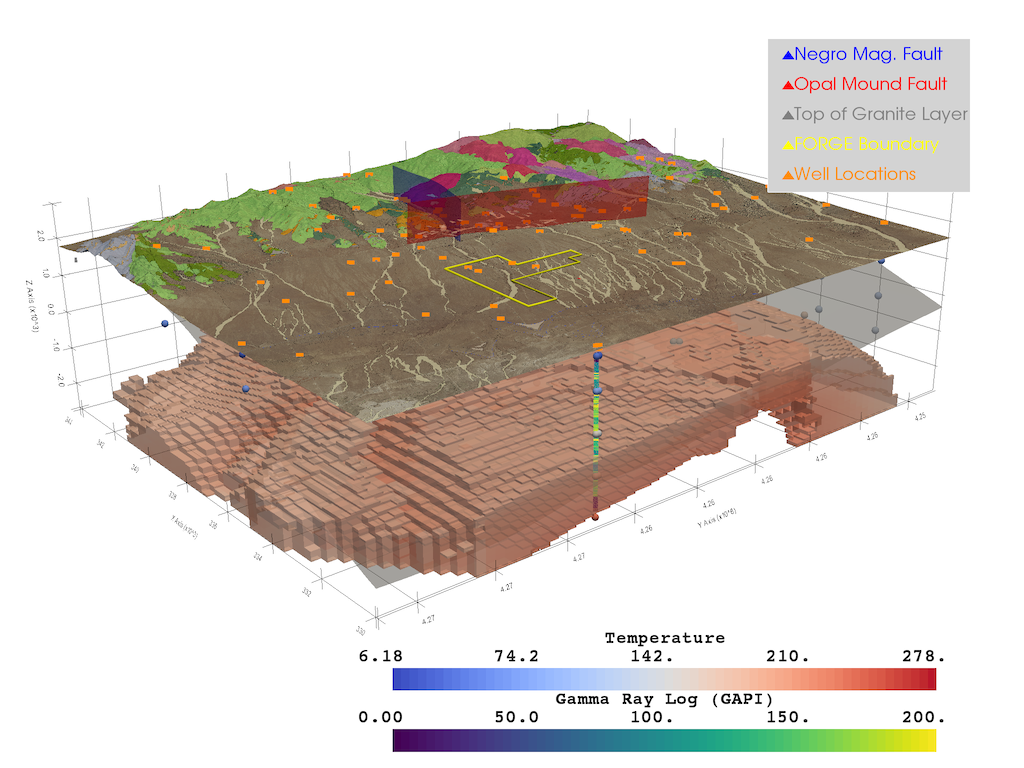
\includegraphics[width=\textwidth]{images/forge-iso}\\

}{
	\section{External Examples}

	
\includegraphics[width=\textwidth]{images/logo-big}\\
 
	pyFBS is a Python package for Frequency Based Substructuring, Transfer Path Analysis and also, as a new addition, multi-reference modal identification.

	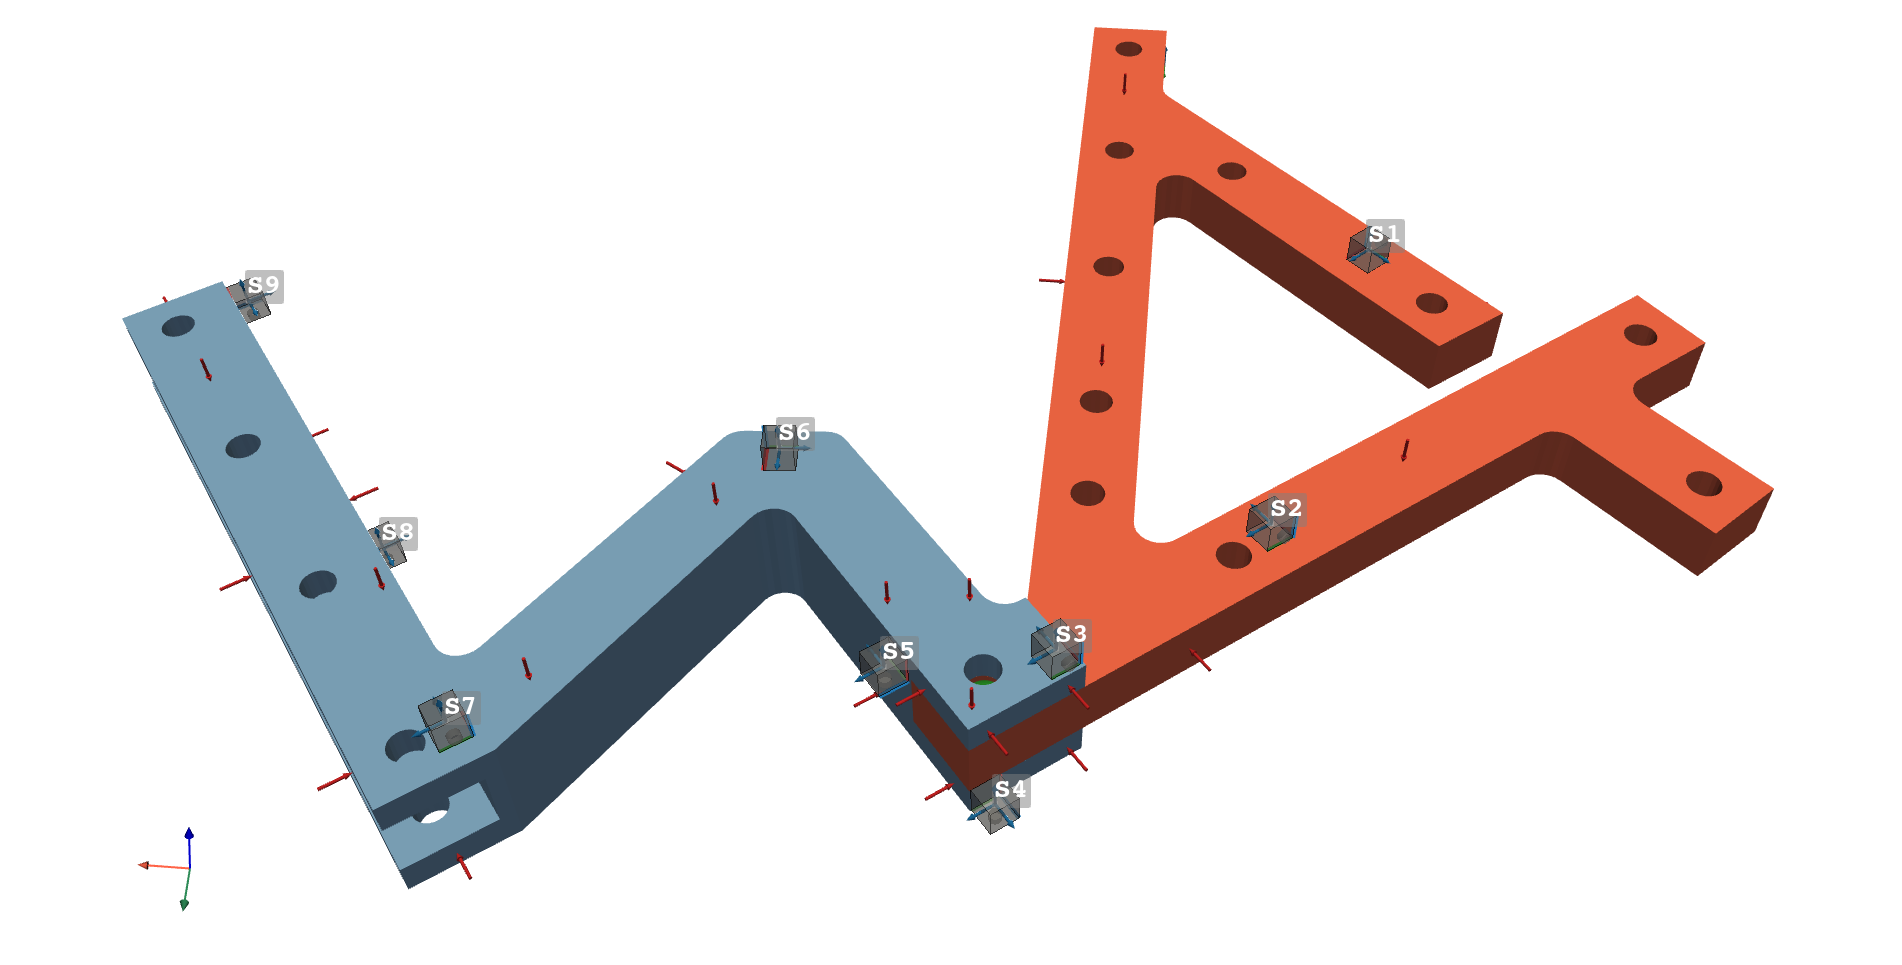
\includegraphics[width=\textwidth]{images/figure}\\

	\qrcode{images/qrcode-pyfbs}{images/smartphoneBlack}{
		\textbf{Take a picture} to
		\\download the full paper
	}\\

	\vspace{60pt}

	
\includegraphics[width=\textwidth]{images/geovistalogo}\\

	Cartographic rendering and mesh analytics powered by PyVista

	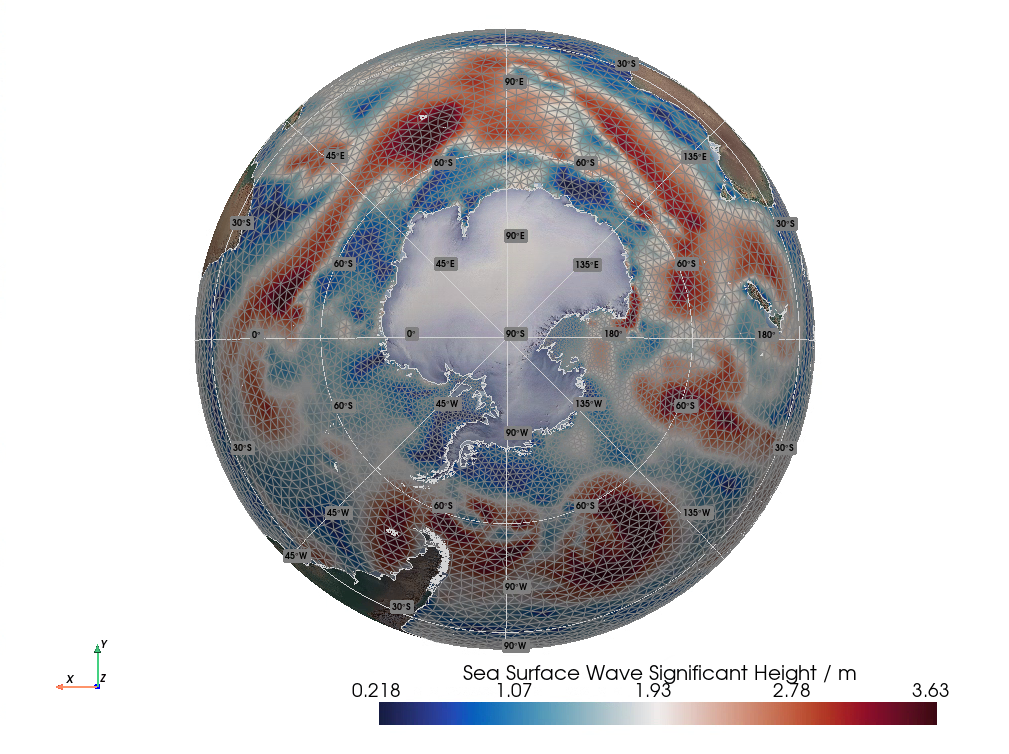
\includegraphics[width=\textwidth]{images/ww3-tri}\\

	\qrcode{images/qrcode-geovista}{images/smartphoneBlack}{
		\textbf{Take a picture} to
		\\visit the GeoVista website
	}\\

	\vspace{60pt}

	\doclicenseLongText\\

	\begin{center}
		\doclicenseImage
	\end{center}

}
\end{document}
